\chapter{Double buffer}\label{chapter:Double buffer}
%What did we want to test?
%How did we want to test?
%What did we expect to observe?
%What results did we observe?
%What are conclusions?

The main idea of the first task is to get rid off blocking operation while sending element of Jacobian matrix to the "server" (NuT). It allows the host application to come back to computation as soon as possible and overlap communication part with computations.\par
execute - tell the server (NUT) what procedure we want to perform next
\begin{lstlisting}[language=C]
// Jacobian Update - Pseudocode
class nut {
	...
	void execute(int entity, int tag) {
		int command[2] = {entity, tag};
		MPI_Send(command, 2, MPI_INT, nut_rank, ...);
	}
	
	...
	void set_matrix_values(double *columns,
				  double *rows,
				  double *values,
				  int length) {
		execute(entity, set_matrix_value);
		MPI_Bcast(columns, length, MPI_INT, host_rank, ...);
		MPI_Bcast(rows, length, MPI_INT, host_rank, ...);
		MPI_Bcast(values, length, MPI_DOUBLE, host_rank, ...);
	}
	...
}

void ComputeJacobian(int problem_size,/*paramenters*/) {

	bool UpdateJacobian = false;
	int num_colors, *indices, *arr_lengths, *arr_pointers;
	
	int *columns, *rows;
	double *values,
		
	// perform analysis to decide whether the current
	// Jacobian matrix is really too old

	if (UpdateJacobian)	{
		// request NuT to compute coloring
		// NuT returns num_colors, *indices, *arr_lengths, *arr_pointers
		
		// allocate resources
		columns = (int*)calloc(problem_size, sizeof(int));
		rows = (int*)calloc(problem_size, sizeof(int));
		values = (double*)calloc(problem_size, sizeof(double));
		
		for (int color = 0; color < num_colors; ++color) {
		
			int length = arr_lengths[color];
			int ptr = arr_pointers[color];
			HOST_perform_perturbation(color,
						     &indices[ptr],
						     &columns,
						     &rows,
						     &values,
						     length,);
						     
			nut.set_matrix_values(&columns, &rows, &values, length);
		}
		
		// release resources
		free(columns); free(rows); free(values);
	} 
}
\end{lstlisting}


"PBIST v.1" - benchmark description\\


"PBIST v.2" - benchmark description\\





%description of IBT benchmark
At the next step we wanted to test whether non-blocking broadcast operation worked in opneMPI 3.1 for both C and Fortran languages. As we discussed above it was not a case for openMPI 2.0. To proceed further we designed another benchmark called Ibcast Test (IBT) for that purpose.\par
The benchmark measures communication time of the sender and it allows to put the sender into sleep for a while right after non-blocking broadcast function call. The user can set up sleeping time via a command-line argument according to the needs.\par

At the benign we measured communication time with zero sleeping (time) in order to find out pure communication time. In that case there is no difference between blocking and non-blocking broadcast operations but this information allows us to adjust sleeping time for further tests. Knowing pure communication time, few tests were performed with different values of sleeping time, namely: 25\%, 50\%, 75\%, 100\%, 125\% of pure communication time. The results of these are represented in figures ... and ...\par

\begin{lstlisting}[language=C]
// IBT Pseudocode
int main(int argc, char *argv[]) {
	
	return 0;    
}
\end{lstlisting}

To get some reference of non-blocking broadcast performance we slightly modified "IBT" benchmark to use blocking broadcast. The result of that can be seen in figure ... and ...\par

At the first glance we can see that non-blocking operation works as expected (figures ... and ...) and it slightly better in comparison to blocking broadcast. However, the first pick which we will call "warm-up" penalty attracted our attention in both cases and we wanted to find out the nature of that effect.\par

Analyzing the source code we can clearly see that it happens every time when we call the "test" function regardless of value of sleeping time. The refinement strategy was to put the "test" function in a for-loop and call it several time during a test. To reduce the number of overall tests we decided to perform a run only for zero sleeping time case because, as we can see from figures ... and ..., the same effect occurs for all cases regardless of sleeping time value. 

\medskip
\emph{description of IBT benchmark}\\
\emph{pseudo code}
\medskip




There are two case to allocate a user MPI buffer on either heap or stack.


In case of "heap" it leads to a penalty each time when we reallocate the user buffer. Basically whenever we pass a pointer with a new address to the begging of an array we have so-called "warm-up" penalty which can be seen in figure. 


\begin{figure}[htpb]
\begin{multicols}{2}
  \centering
  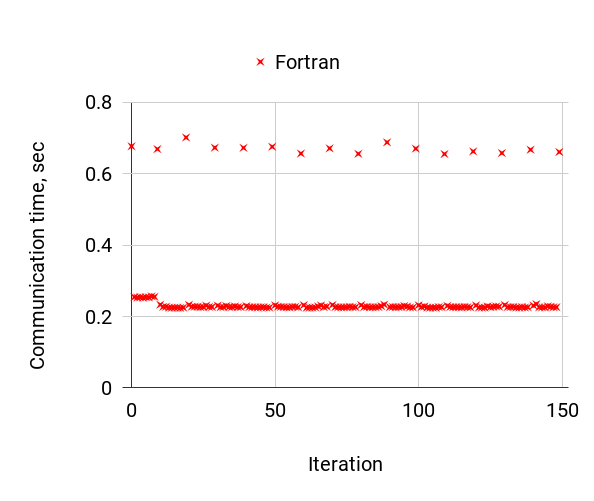
\includegraphics[width=0.5\textwidth]{figures/MPI_Ibcast-performance-Fortran-language.png}\par
   
   \centering
  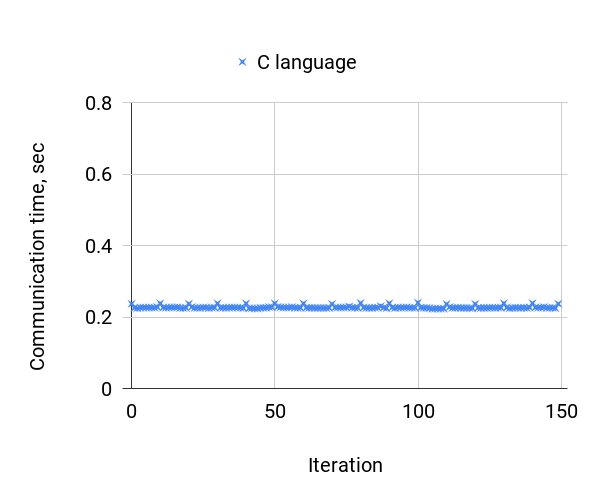
\includegraphics[width=0.5\textwidth]{figures/MPI_Ibcast-performance-C-language.png}\par
\end{multicols}
\caption{An example of application coupling}
\end{figure}


It is worth noticing that effect does not happen with an array allocated on stack. This approach only leads to one initial "warm-um" penalty at the first function call as it can be seen in figure [2]. After that communication time reduces by the factor of [something] in case of "manni" cluster. 

In general several runs were performed on different clusters ("manni" and "SuperMUC") with different compilers and MPI distributions (ibm, intel, openMPI) and we could see the same typical behavior. The only difference that could be observed was the difference in absolute values of communication time.


The outcome of that benchmark is the following: 
\begin{enumerate}
	\item a user MPI buffer must be allocated on heap as least as possible to avoid "warm-up" penalty.
	\item  Moreover, in general non blocking broadcast implementation is two times faster in contrast to blocking one in case of "manni" cluster and the "warm-up" penalty is [x15] smaller in case of non-blocking broadcast.
\end{enumerate}
 

It should be pointed out the result of the second clause is particular valid for the current "manni" configuration and current openMPI version (3.1). The results may be different in the future. Thus, we have to preserve "IBT" benchmark for the future test to examine, for instance, a new openMPI version. 


The next step was to make a copy of Jacobian matrix pattern and use to in our "PBIST" benchmark. The intent of that was to measure possible performance improvement. Previous tests were done only for so-called square, rectangular [, linear, paraboloid] patterns where size of a vector was always constant [or changing according to a corresponding law(equation)]. At that point we wanted to make one step closer towards a real (practical) problem. [question that we want to answer whether the pattern in original test was too small that we could not observe any performance gain]



